\documentclass{hw}

\title{Short Essay 3}
\author{MATH 168, Spring 2022}
\date{Due Friday, April 22nd}

\begin{document}


\section*{Short Essay 3}

In this short essay, you'll apply several computational techniques from class to a real-world network. 
This essay involves both coding and writing components. 
Because of this, this essay actually counts under \textbf{both} your project and your homework grades. 
A fully successful short essay will receive both 5 points toward the project grade and 3 points toward the homework grade. 

You can complete this essay using any computational software you choose. 
I can guarantee that it is possible to do everything relatively efficiently in Python with NetworkX. 

\part 

Find a small, undirected, real-world network. 
I suggest browsing the \href{https://icon.colorado.edu/#!/}{Colorado Index of Complex Networks} and choosing one that interests you. 
Your network should be relatively small -- 50 nodes or so is a good size. 
Download your network, save it somewhere where you can find it, and load it into your software of choice. 

\part 

Compute the \emph{degree distribution} of your network, and plot it as a histogram or scatterplot. 
An example of the kind of plot I am looking for is on the bottom right in \href{https://networkx.org/documentation/stable/auto_examples/drawing/plot_degree.html}{this NetworkX demo}. 
Please make sure to label your axes! 

\part 

Recall the idea of \href{http://www.philchodrow.com/intro-networks/chapters/measurement.html#triadic-closure-transitivity}{triadic closure} from lecture. 
Broadly, triadic closure is the idea that triangles are common in the network when compared to what would be expected by random chance. 

\begin{itemize}
    \item Compute the global clustering coefficient (also called the \emph{transitivity}) of your network. 
    You don't have to do this ``by hand;'' most software packages can do this for you. 
    In NetworkX, the relevant function is \texttt{networkx.transitivity()}. 
    \item Compute the average degree of your network, and create an Erd\H{o}s-R\'enyi random graph with approximately the same average degree. 
    Compute the global clustering coefficient of the Erd\H{o}s-R\'enyi graph. 
    How large is the clustering coefficient in your chosen network when compared to the ER graph? 
    Would you say that your graph exhibits triadic closure? 
\end{itemize}
You don't need to create a visualization for this part, but please plan to explain your results in writing (see below). 

\part 

Recall the \href{http://www.philchodrow.com/intro-networks/chapters/measurement.html#betweenness-centrality}{betweenness centrality} as a way of measuring the importance of nodes by quantifying how many geodesic paths pass through them. 
Compute the betweenness centrality of all the nodes in your network. 

\begin{hint}
    I do \textbf{not} recommend trying to do this with your own hand-coded solution. 
    Instead, find a function that does this for you in your favorite software! 
\end{hint}

You don't need to produce a visualization for this part. 
Save your result for now. 

\part 

Recall the idea of \href{http://www.philchodrow.com/intro-networks/chapters/measurement.html#betweenness-centrality}{community structure} in graphs. 
We've talked briefly about the idea that finding eigenvectors with small eigenvalues of the graph Laplacian matrix $\mathbf{L}$ might be a good way to find community structure. 
You don't have to take that approach; instead, find \emph{any} algorithm for community detection or graph partitioning implemented in your preferred software and apply it to your network. 
If you are using NetworkX, I suggest the modularity-maximization method called the \emph{Louvain method}. 
This function is implemented in NetworkX as  
\begin{quote}
    \texttt{networkx.algorithms.community.louvain\_communities()}
\end{quote}
as one that usually leads to usefully visualizable results. 
Please briefly explain what your algorithm does, and why that's a reasonable thing to do. 
You don't have to go into much mathematical detail. 
Newman 14.2 gives some discussion of modularity maximization methods in 14.2.


\part 

Create an attractive plot of your network in which the size of each node reflects its betweenness centrality (from Part (d)) and the color of each node reflects its community (from Part (e)). 
An example of a successful visualization is shown in \Cref{fig:example}. 

\begin{figure}
    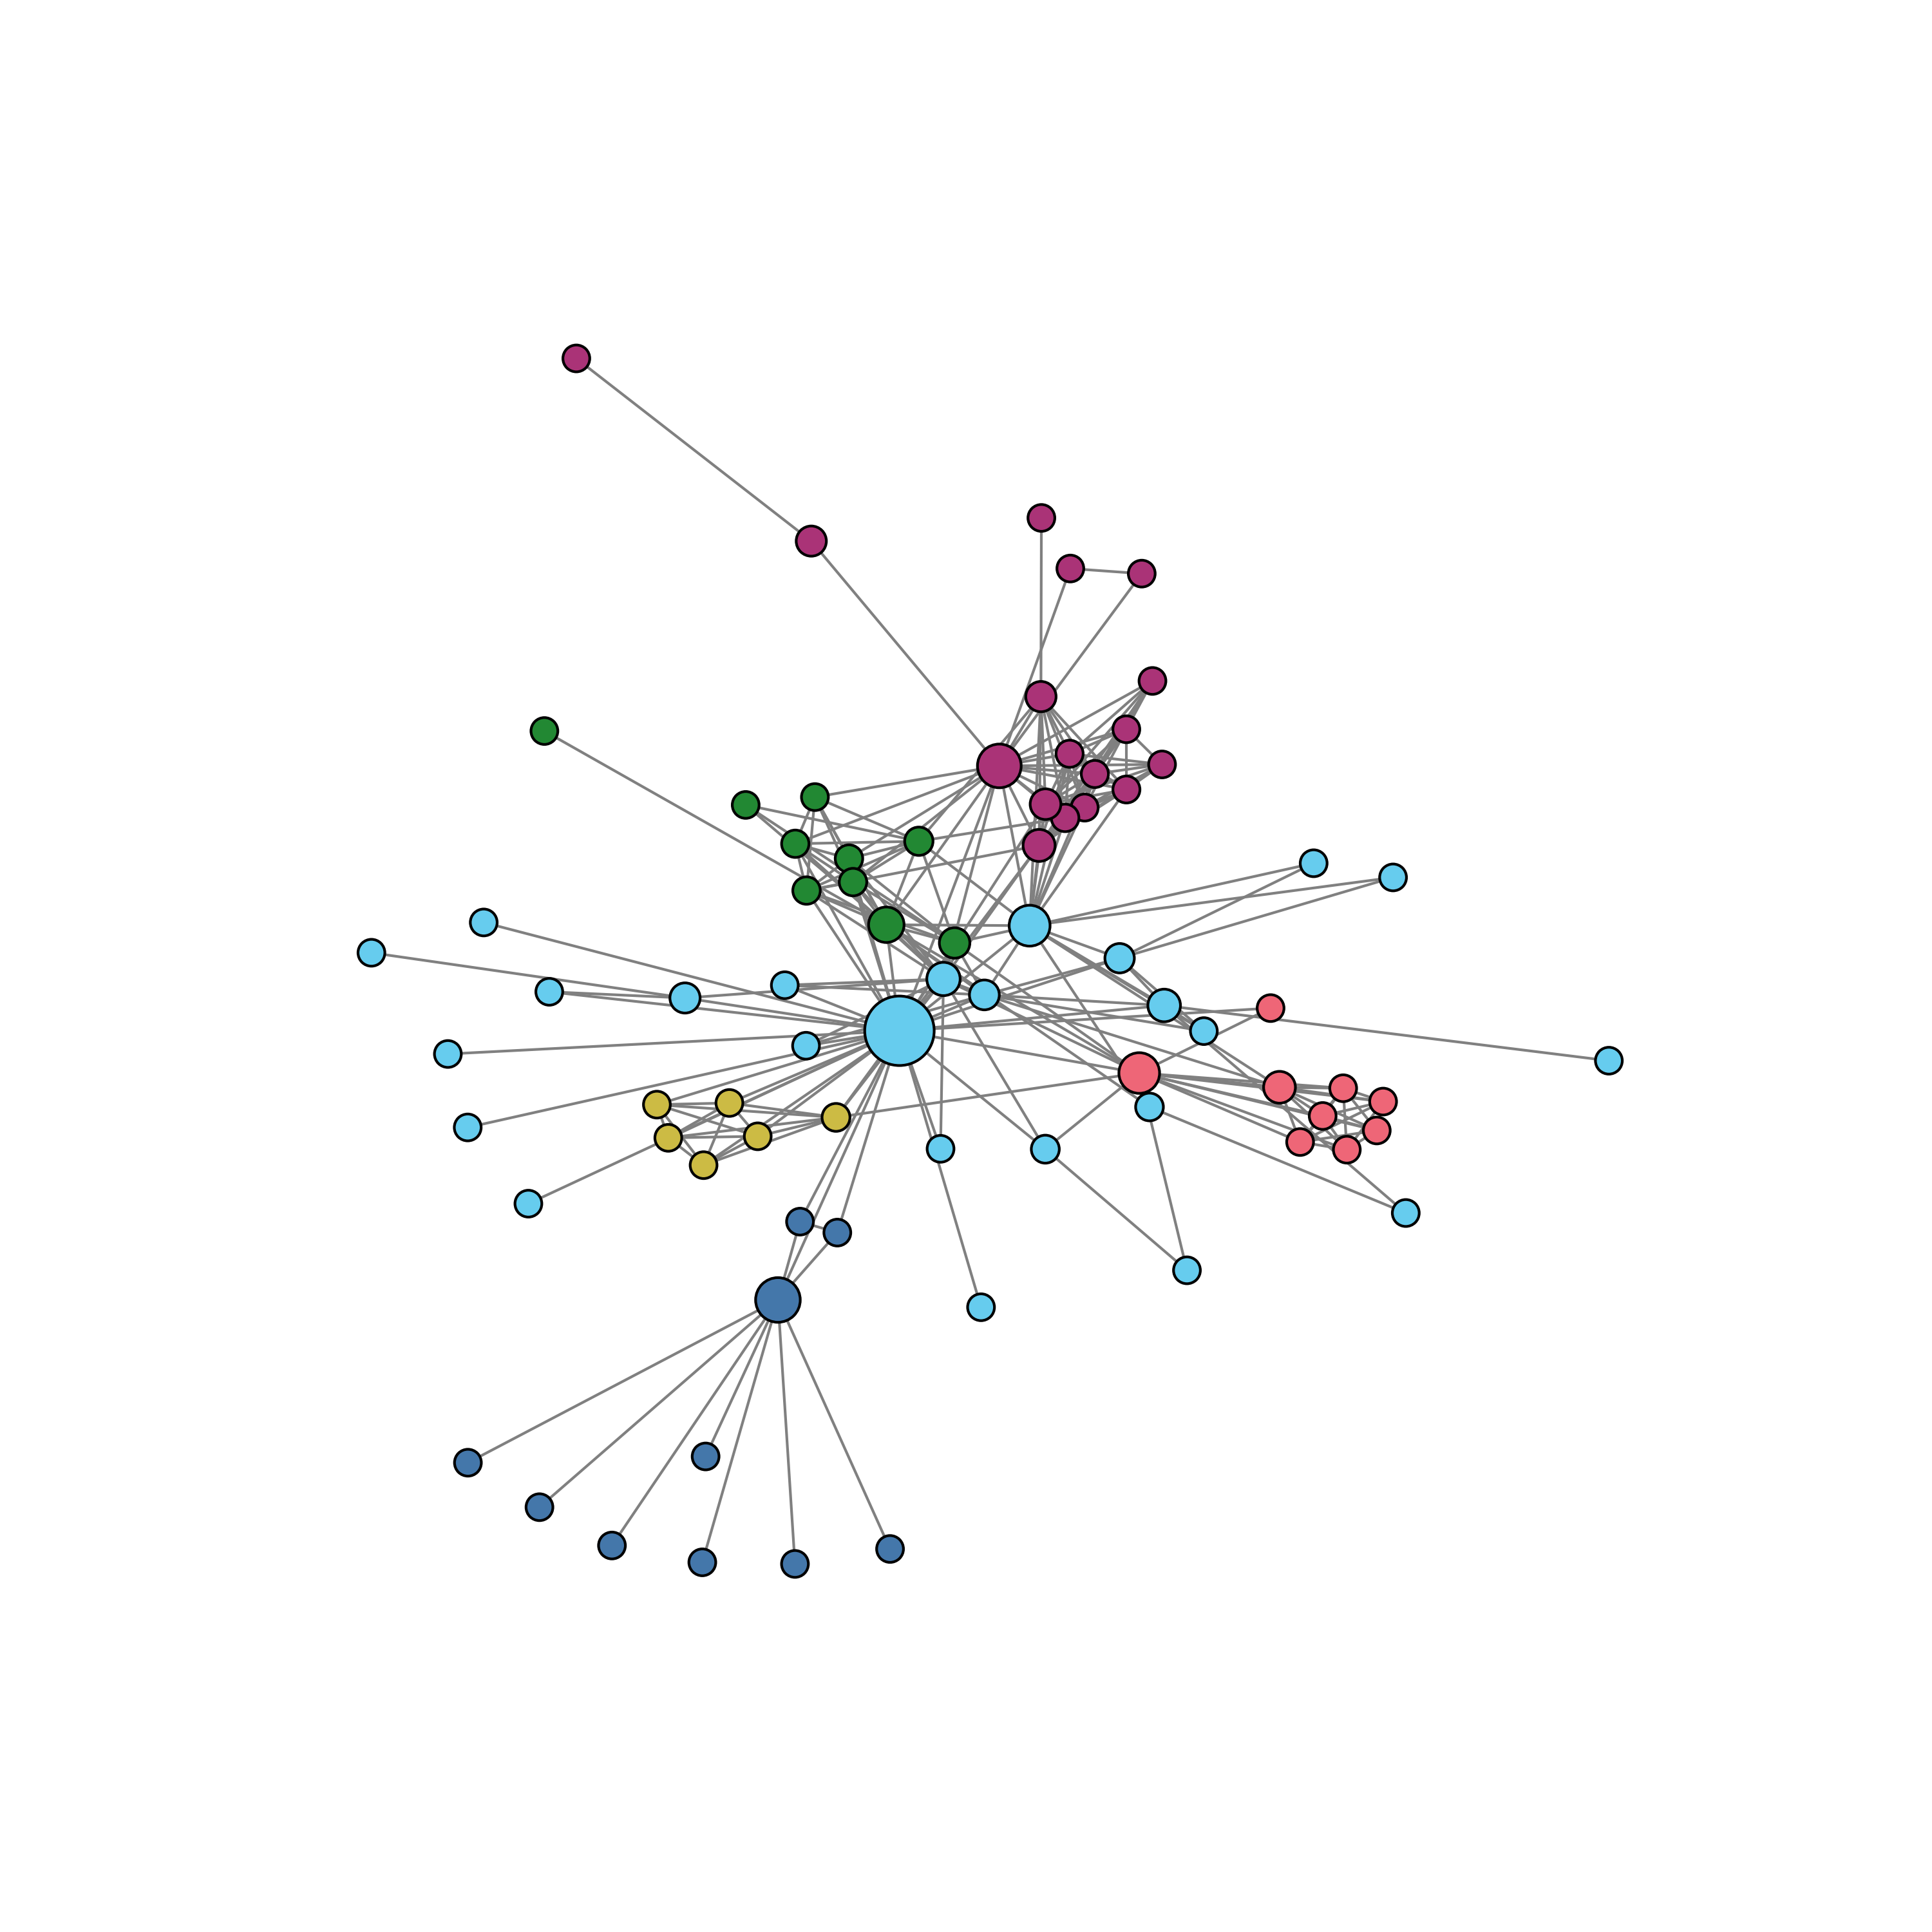
\includegraphics[width=\textwidth]{img/mis-example.png}
    \caption{An example of a network visualization in which node size corresponds to betweenness centrality and node color corresponds to communities as computed by an algorithm.}\label{fig:example}
\end{figure}

\part 

Using \LaTeX, write an essay of between 500 and 1000 words about your network. 
Your essay should include discussion of your findings in the previous parts. 
The following sequence of paragraphs is recommended: 

\begin{itemize}
    \item Explain where your network came from and what the nodes and edges mean. 
    If your network was originally produced by researchers, cite the source in which they published it. 
    \item Discuss the degree distribution of your network, and show the plot from Part (b), with a caption. 
    Discuss the clustering coefficient, and comment on the comparison to the random ER graph (from Part (c)). 
    Based on some of Newman's discussion of the clustering coefficient in Chapter 7.3, is your network one in which you would expect a large clustering coefficient? 
    \item Show your beautiful network plot from Part (f). 
    Comment on the visual appearance of the betweenness centrality: does it look like there are a few very central nodes, or do most of the nodes look roughly equally central? 
    Comment also on the visual appearance of the communities found by the clustering algorithm. 
    Do they look visually reasonable? 
    Based on how the data for this network was collected, would you expect to see significant community structure? 
    \item In your final paragraph, include some brief reflection on what you have learned about your network. 
\end{itemize}


\section*{Grading}

Here's how grading works for this assignment. 
\begin{itemize}
    \item Turn in your \textbf{code} and \textbf{outputs} as part of your submission for Homework 3. 
    If you worked in a Jupyter Notebook, a pdf printout of the notebook that includes both code and visualizations is sufficient. 
    \item Turn in your \textbf{essay} as its own submission, under Short Essay 3. 
\end{itemize}

\end{document}